\documentclass[11pt]{article}
\usepackage[margin=0.86in]{geometry}
\usepackage{amsmath,amssymb,mathtools,amsthm}
\usepackage{booktabs,longtable,array,tabularx,multirow}
\usepackage{graphicx,float,caption,subcaption}
\usepackage{hyperref,xcolor,listings,microtype}
\usepackage[T1]{fontenc}
\usepackage{lmodern}
\usepackage{enumitem}
\usepackage{fancyhdr}
\usepackage{lastpage}
\usepackage{bm}
\hypersetup{colorlinks=true,linkcolor=black,urlcolor=blue,citecolor=black,pdftitle={Projector Special-Function Registry},pdfauthor={Komorebi P.},pdfsubject={},pdfkeywords={}}
\pagestyle{fancy}
\fancyhf{}
\lhead{Projector Special-Function Registry}
\rhead{Komorebi P.}
\cfoot{\thepage\ of \pageref{LastPage}}
\setlength{\headheight}{14pt}
\newtheorem{theorem}{Theorem}[section]
\newtheorem{proposition}[theorem]{Proposition}
\newtheorem{lemma}[theorem]{Lemma}
\newtheorem{corollary}[theorem]{Corollary}
\theoremstyle{definition}
\newtheorem{definition}[theorem]{Definition}
\newtheorem{example}[theorem]{Example}
\theoremstyle{remark}
\newtheorem{remark}[theorem]{Remark}
\newcommand{\BNj}{\mathcal B_{N,j}}
\newcommand{\EE}{\mathsf E}
\newcommand{\Sec}{\mathsf{Sec}}
\newcommand{\Tan}{\mathsf{Tan}}
\newcommand{\CE}{\mathsf{CE}}
\newcommand{\Zb}{\mathfrak Z}
\newcommand{\C}{\mathbb C}
\newcommand{\Q}{\mathbb Q}
\newcommand{\Z}{\mathbb Z}
\newcommand{\Fp}{\mathbf F_p}
\newcommand{\ord}{\operatorname{ord}}
\newcommand{\Res}{\operatorname{Res}}
\newcommand{\Tr}{\operatorname{Tr}}
\newcommand{\sech}{\operatorname{sech}}
\newcommand{\Li}{\operatorname{Li}}
\newcommand{\status}[1]{\textsf{#1}}
\lstset{basicstyle=\ttfamily\footnotesize,breaklines=true,frame=single,columns=fullflexible,showstringspaces=false}
\begin{document}

\begin{center}
{\LARGE\bfseries Projector Special-Function Registry}\par\vspace{0.35em}
{\large Scalar families, polynomial companions, $p$-adic avatars, and operator-valued extensions}\par\vspace{0.8em}
{\large Komorebi P.}\par
\end{center}

\begin{abstract}
The projector calculus does generate special-function families, but not every projected expression should be advertised as a new special function.  The block sections of the exponential are classical multisections and generalized hypergeometric functions; the same is true of several boundary cases involving Euler, Bernoulli, Appell, and higher-order Euler theory.  The calculus becomes distinct when it organizes normalized reciprocals, reciprocal-power towers, logarithmic-derivative companions, congruential inverse sections, packetwise Appell polynomials, zero-spectrum zeta functions, and $p$-adic block avatars inside one exact algebra.

This registry documents every canonical function family presently supported by the transfer-block corpus.  Each entry receives a definition, differential or recurrence law, product or refinement law, classical specialization, analytic status, arithmetic meaning, and novelty status.  The purpose is not to make a priority claim by naming a formula.  It is to identify which objects are classical sections, which are mathematically substantive derived families, which are credible candidates for new named functions, and which remain operator schemas rather than scalar special functions.
\end{abstract}

\tableofcontents
\clearpage

\section{What it means for the calculus to generate a special function}

A coefficient projector creates infinitely many functions.  If
\[
F(z)=\sum_{m\ge0}a_m\frac{z^m}{m!},
\qquad \omega=e^{2\pi i/N},
\]
then
\[
\BNj F(z)
=\sum_{n\ge0}a_{Nn+j}\frac{z^{Nn+j}}{(Nn+j)!}
=\frac1N\sum_{\ell=0}^{N-1}\omega^{-j\ell}F(\omega^\ell z).
\]
Thus every seed function produces $N$ residue sections.  Repeating this for every analytic seed gives an infinite construction class, so a literal list of every output would be neither finite nor useful.

This document uses a stricter criterion.  A family belongs in the registry when it has at least three of the following:
\begin{enumerate}[label=(\roman*)]
\item an intrinsic parameterized definition;
\item a differential, difference, or functional equation;
\item a stable product, inverse, composition, or refinement law;
\item a coefficient recurrence or finite combinatorial formula;
\item a recognizable analytic continuation, pole, or zero structure;
\item a nontrivial arithmetic or $p$-adic interpretation;
\item a classical specialization that fixes normalization.
\end{enumerate}

Four status labels are used.
\begin{description}[style=nextline]
\item[Classical boundary.] The scalar function already belongs to established special-function theory, although the projector interpretation may be useful.
\item[Explicit derived family.] The calculus gives a complete definition and laws, but a literature audit may reveal equivalent prior notation.
\item[Candidate-new family.] The family appears structurally distinct and deserves a priority search; no claim of novelty is made here.
\item[Operator or construction schema.] The object is mathematically useful but is not one scalar special function.
\end{description}

The existing transfer-block source already records five core families: transfer exponentials, transfer secants, congruential Euler blocks, spectral block zeta functions, and block-Appell polynomials.  The larger corpus adds logarithmic-derivative companions, higher reciprocal powers, higher-order Euler transfer, theta polynomials, $p$-adic avatars, resolvent packets, and nonlinear jet families.  The present registry consolidates them and separates their statuses.

\section{The universal block-section operator}

\begin{definition}[Residue section]
For $0\le j<N$, define
\[
\BNj F(z)=\frac1N\sum_{\ell=0}^{N-1}\omega^{-j\ell}F(\omega^\ell z).
\]
\end{definition}

\begin{proposition}[Projection and reconstruction]
For analytic $F$,
\[
\mathcal B_{N,i}\mathcal B_{N,j}=\delta_{ij}\mathcal B_{N,j},
\qquad
\sum_{j=0}^{N-1}\mathcal B_{N,j}=I.
\]
If $F,G$ are analytic, then
\[
\mathcal B_{N,r}(FG)
=\sum_{a+b\equiv r\pmod N}
(\mathcal B_{N,a}F)(\mathcal B_{N,b}G).
\]
\end{proposition}

\begin{proof}
The root-of-unity orthogonality identity
\[
\frac1N\sum_{\ell=0}^{N-1}\omega^{\ell(m-j)}
=\mathbf 1_{m\equiv j\, (N)}
\]
selects the desired coefficients.  The product law follows by sorting the Cauchy product according to the sum of residue classes.
\end{proof}

\begin{remark}
This construction is classical as a multisection or root-of-unity filter.  The new mathematical content of the projector calculus is not the existence of the filter itself, but the systematic closure, refinement, inverse, arithmetic, nonlinear, and operator laws built around it.
\end{remark}

\section{Transfer exponentials}

\begin{definition}
For $0\le j<N$ and $\lambda\in\C$, define
\[
\boxed{
\EE_{N,j}(\lambda z)
=\mathcal B_{N,j}(e^{\lambda z})
=\sum_{n\ge0}\frac{(\lambda z)^{Nn+j}}{(Nn+j)!}.
}
\]
\end{definition}

The root-filter and generalized hypergeometric forms are
\[
\EE_{N,j}(\lambda z)
=\frac1N\sum_{\ell=0}^{N-1}\omega^{-j\ell}e^{\lambda\omega^\ell z},
\]
\[
\EE_{N,j}(\lambda z)
=\frac{(\lambda z)^j}{j!}
{}_0F_{N-1}\!\left(;
\mathcal P_{N,j};\frac{(\lambda z)^N}{N^N}\right),
\]
where
\[
\mathcal P_{N,j}
=\left\{\frac{j+1+q}{N}:0\le q<N\right\}\setminus\{1\}.
\]

\begin{proposition}[Differential cycle]
With indices read modulo $N$,
\[
\frac{d}{dz}\EE_{N,j}(\lambda z)
=\lambda\EE_{N,j-1}(\lambda z),
\qquad
\frac{d^N}{dz^N}\EE_{N,j}(\lambda z)
=\lambda^N\EE_{N,j}(\lambda z).
\]
Moreover,
\[
\sum_{j=0}^{N-1}\EE_{N,j}(\lambda z)=e^{\lambda z}.
\]
\end{proposition}

\begin{proposition}[Addition law]
\[
\EE_{N,r}(x+y)
=\sum_{a+b\equiv r\pmod N}
\EE_{N,a}(x)\EE_{N,b}(y).
\]
\end{proposition}

The addition law shows that the vector
\[
\bm{\EE}_N(z)=
(\EE_{N,0}(z),\ldots,\EE_{N,N-1}(z))^T
\]
is a finite-dimensional representation of the additive group under cyclic convolution.

\begin{figure}[H]
\centering
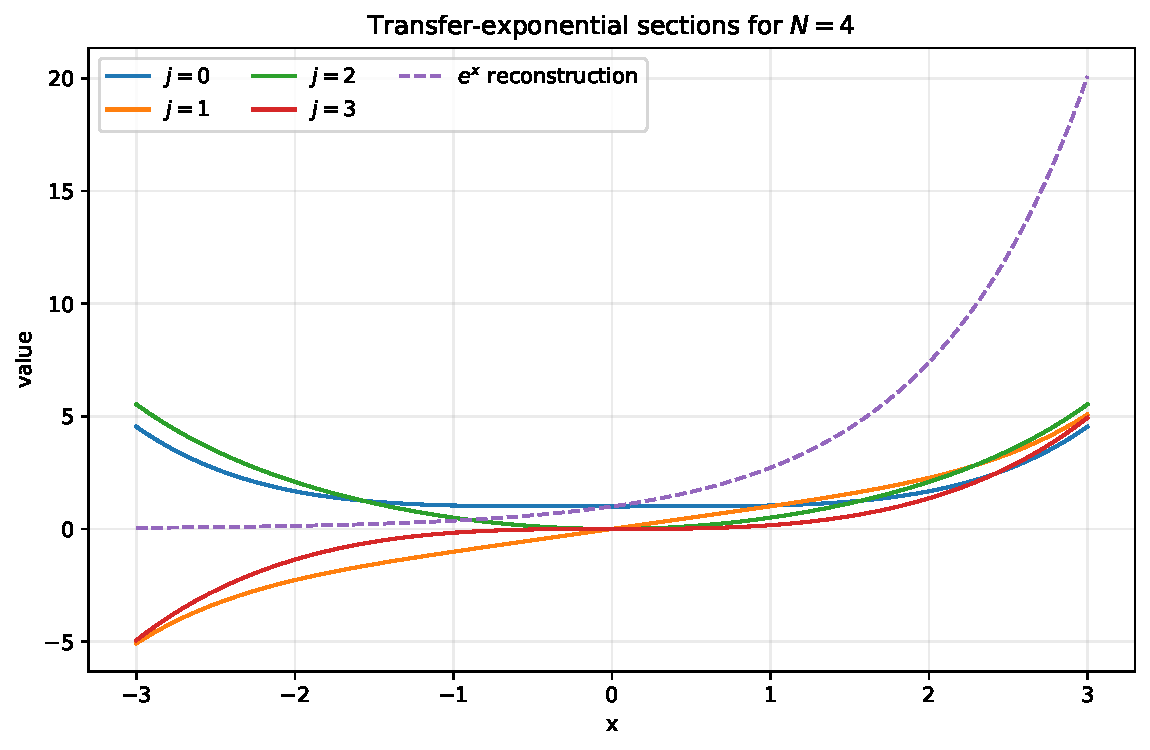
\includegraphics[width=.88\linewidth]{figures/01_transfer_exponentials_N4.pdf}
\caption{The four residue sections reconstruct $e^x$ exactly.  Their individual shapes are not independent accidents; they are the components of one cyclic differential system.}
\end{figure}

\paragraph{Status.}
These functions are classical exponential multisections and hypergeometric functions.  Their role as the universal seed of the transfer calculus is important, but the scalar functions themselves should not be claimed as new.

\section{Universal transfer denominators}

\begin{definition}
\[
\boxed{
D_N(z)=\sum_{n\ge0}(-1)^n\frac{z^{Nn}}{(Nn)!}.
}
\]
\end{definition}

If $\lambda^N=-1$, then
\[
D_N(z)=\EE_{N,0}(\lambda z)
=\frac1N\sum_{\mu^N=-1}e^{\mu z}.
\]
Consequently,
\[
D_N^{(N)}(z)=-D_N(z),
\qquad D_N(0)=1,
\qquad D_N^{(k)}(0)=0\quad(1\le k<N).
\]
It also has the hypergeometric form
\[
D_N(z)
={}_0F_{N-1}\!\left(;
\frac1N,\frac2N,\ldots,\frac{N-1}{N};
-\frac{z^N}{N^N}\right).
\]

Important low-order cases are
\[
D_2(z)=\cos z,
\]
\[
D_3(z)=\frac13\sum_{\lambda^3=-1}e^{\lambda z},
\]
\[
D_4(z)=\cos(z/\sqrt2)\cosh(z/\sqrt2).
\]

\begin{figure}[H]
\centering
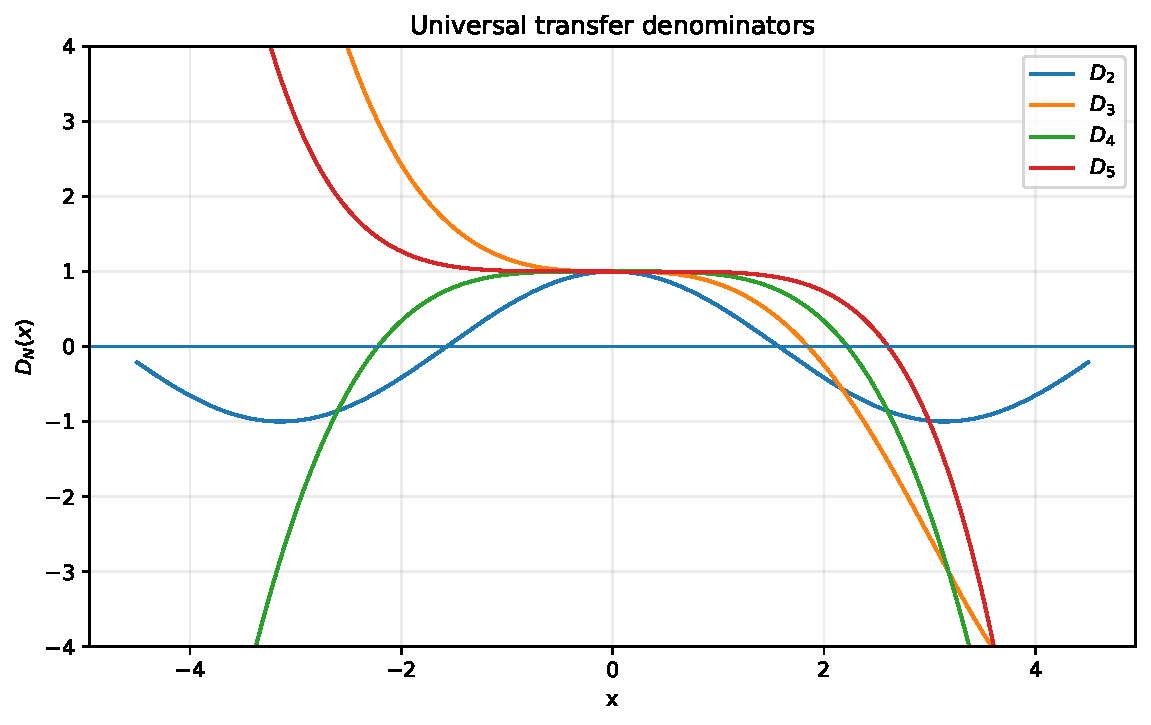
\includegraphics[width=.88\linewidth]{figures/02_transfer_denominators.pdf}
\caption{Several members of the denominator family.  Their zeros control the poles and coefficient growth of the reciprocal families.}
\end{figure}

\paragraph{Status.}
$D_N$ is a classical hypergeometric/exponential-polynomial object.  The universal normalization and its use as the denominator of an arithmetic reciprocal tower are the distinctive parts of the present framework.

\section{Transfer secants}

\begin{definition}[Integer order]
For $r\in\Z_{\ge0}$,
\[
\boxed{
\Sec_N^{[r]}(z)=D_N(z)^{-r}.
}
\]
Write
\[
\Sec_N^{[r]}(z)
=\sum_{n\ge0}A_N^{[r]}(n)\frac{z^{Nn}}{(Nn)!}.
\]
\end{definition}

For complex $\alpha$, the same expression defines a germ at the origin by choosing the branch with value $1$ at $z=0$:
\[
\Sec_N^{[\alpha]}(z)=\exp[-\alpha\log D_N(z)].
\]
It becomes multivalued around zeros when $\alpha\notin\Z$.

\begin{theorem}[Semigroup and coefficient convolution]
\[
\Sec_N^{[r]}(z)\Sec_N^{[s]}(z)=\Sec_N^{[r+s]}(z),
\]
so
\[
A_N^{[r+s]}(n)
=\sum_{q=0}^n
\binom{Nn}{Nq}A_N^{[r]}(q)A_N^{[s]}(n-q).
\]
\end{theorem}

\begin{theorem}[Triangular recurrence]
\[
\sum_{k=0}^n(-1)^k\binom{Nn}{Nk}A_N^{[r]}(n-k)
=A_N^{[r-1]}(n).
\]
For $r=1$,
\[
A_N(n)=\sum_{k=1}^n(-1)^{k+1}\binom{Nn}{Nk}A_N(n-k).
\]
\end{theorem}

\begin{theorem}[Partition form]
Let $M=\sum_i m_i$.  Then
\[
\boxed{
A_N^{[r]}(n)
=(Nn)!\sum_{\sum i m_i=n}
(-1)^{n+M}(r)_M
\prod_{i\ge1}\frac1{m_i!((Ni)!)^{m_i}}.
}
\]
\end{theorem}

\begin{example}
\[
\Sec_2^{[1]}(z)=\sec z,
\qquad
\Sec_4^{[1]}(z)
=\frac1{\cos(z/\sqrt2)\cosh(z/\sqrt2)}.
\]
The first identifies the classical boundary.  The second displays the first genuinely nonclassical-looking member of the family.
\end{example}

\begin{figure}[H]
\centering
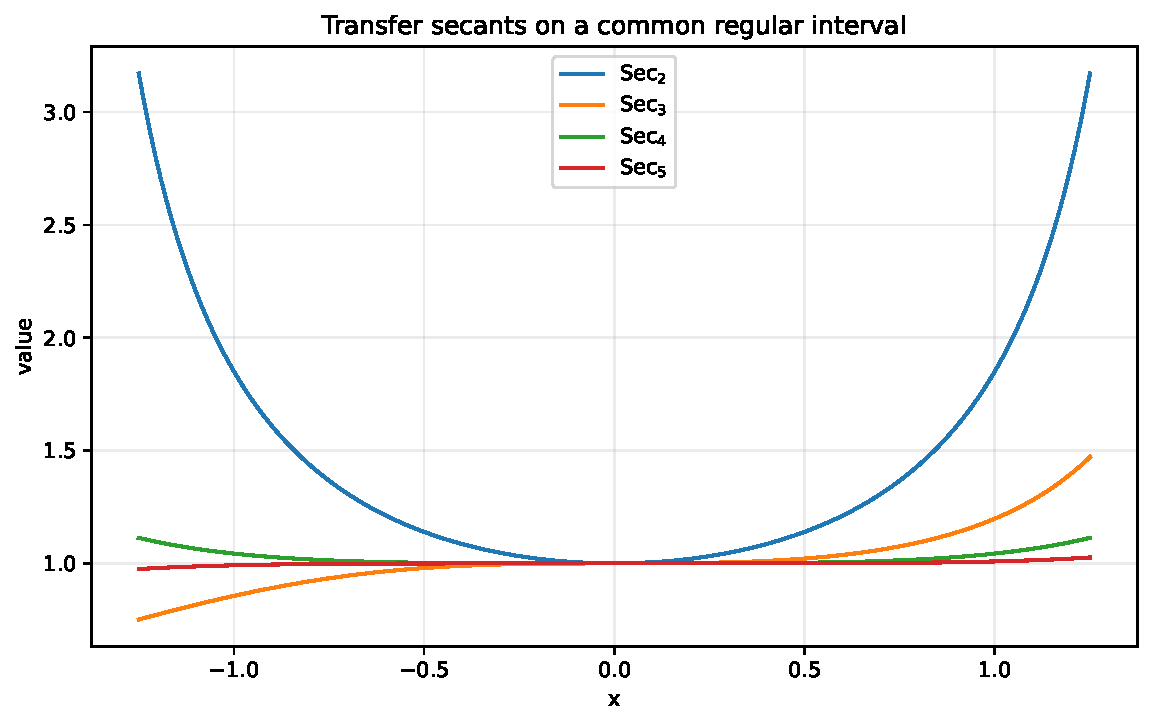
\includegraphics[width=.88\linewidth]{figures/03_transfer_secants.pdf}
\caption{The principal transfer secants on an interval avoiding their first poles.}
\end{figure}

\begin{figure}[H]
\centering
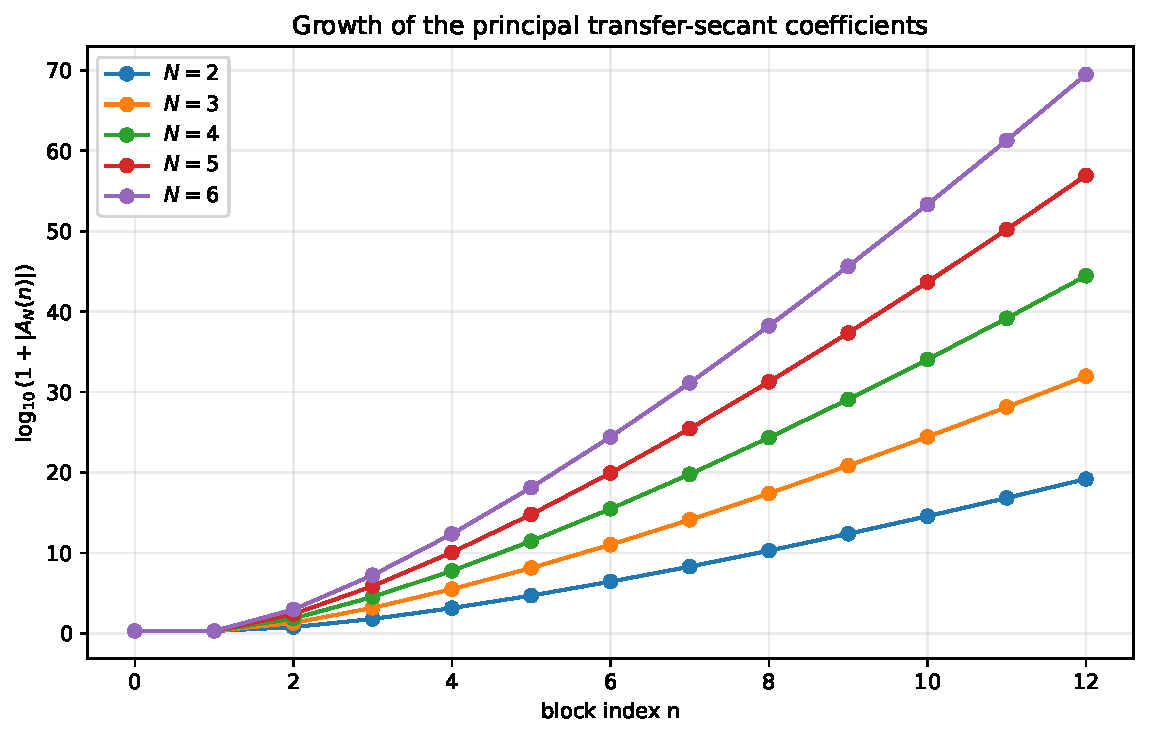
\includegraphics[width=.88\linewidth]{figures/12_secant_coefficient_growth.pdf}
\caption{Coefficient growth is governed by the nearest zero packets of $D_N$.}
\end{figure}

\paragraph{Status.}
The full two-parameter family $(N,r)$, together with its block recurrence, partition formula, arithmetic filtration, and spectral asymptotics, is a strong candidate for a named new family.  A dedicated literature audit is still required before claiming priority.

\section{Transfer tangents and logarithmic-derivative companions}

\begin{definition}
\[
\boxed{
\Tan_N(z)=-\frac{D_N'(z)}{D_N(z)}.
}
\]
\end{definition}

This normalization gives
\[
\Tan_2(z)=\tan z.
\]
It is the infinitesimal generator of the reciprocal-power tower:
\[
\boxed{
\frac{d}{dz}\Sec_N^{[r]}(z)
=r\Tan_N(z)\Sec_N^{[r]}(z).
}
\]
The support has one residue class:
\[
\Tan_N(z)
=\sum_{n\ge0}T_N(n)
\frac{z^{Nn+N-1}}{(Nn+N-1)!}.
\]
The coefficients obey
\[
\boxed{
\sum_{k=0}^n(-1)^k
\binom{Nn+N-1}{Nk}T_N(n-k)=(-1)^n.
}
\]
For $N=2$, this begins
\[
1,2,16,272,7936,\ldots,
\]
the classical tangent-number sequence.

\begin{figure}[H]
\centering
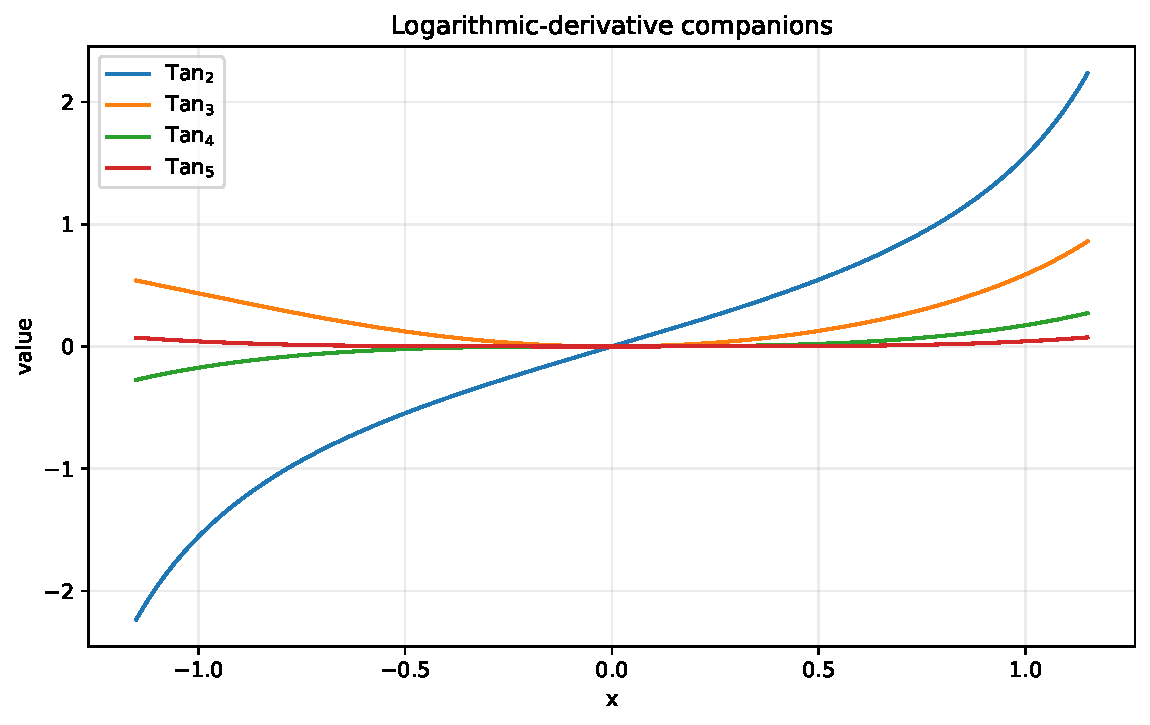
\includegraphics[width=.88\linewidth]{figures/04_transfer_tangents.pdf}
\caption{The logarithmic-derivative companions contain the tangent function at $N=2$ and retain the pole set of the corresponding transfer secant.}
\end{figure}

\paragraph{Status.}
This family is an immediate and fully defined consequence of inverse and logarithmic-derivative closure.  It is a credible derived special-function family, although logarithmic derivatives of exponential polynomials are classical objects in general.

\section{Congruential Euler block functions}

Define the unsigned residue section
\[
S_{N,j}(z)=\sum_{n\ge0}\frac{z^{Nn+j}}{(Nn+j)!}
=\EE_{N,j}(z).
\]

\begin{definition}
\[
\boxed{
\CE_{N,j}(z)
=\frac{z^j/j!}{S_{N,j}(z)}
=\left[{}_0F_{N-1}\!\left(;
\mathcal P_{N,j};\frac{z^N}{N^N}\right)\right]^{-1}.
}
\]
Write
\[
\CE_{N,j}(z)
=\sum_{n\ge0}E_{Nn}^{(N,j)}\frac{z^{Nn}}{(Nn)!}.
\]
\end{definition}

\begin{theorem}[Triangular inverse system]
\[
\boxed{
\sum_{q=0}^n
\binom{Nn+j}{Nq}E_{Nq}^{(N,j)}
=\delta_{n0}.
}
\]
Equivalently, for $n\ge1$,
\[
E_{Nn}^{(N,j)}
=-\frac{\sum_{q=0}^{n-1}\binom{Nn+j}{Nq}E_{Nq}^{(N,j)}}{\binom{Nn+j}{Nn}}.
\]
\end{theorem}

The logarithmic companion is
\[
\Tan_{N,j}^{\mathrm{CE}}(z)
=-\frac{d}{dz}\log\CE_{N,j}(z)
=\frac{S_{N,j}'(z)}{S_{N,j}(z)}-\frac{j}{z},
\]
where the singularity at the origin is removable because $S_{N,j}(z)=z^j/j!+O(z^{N+j})$.

\begin{figure}[H]
\centering
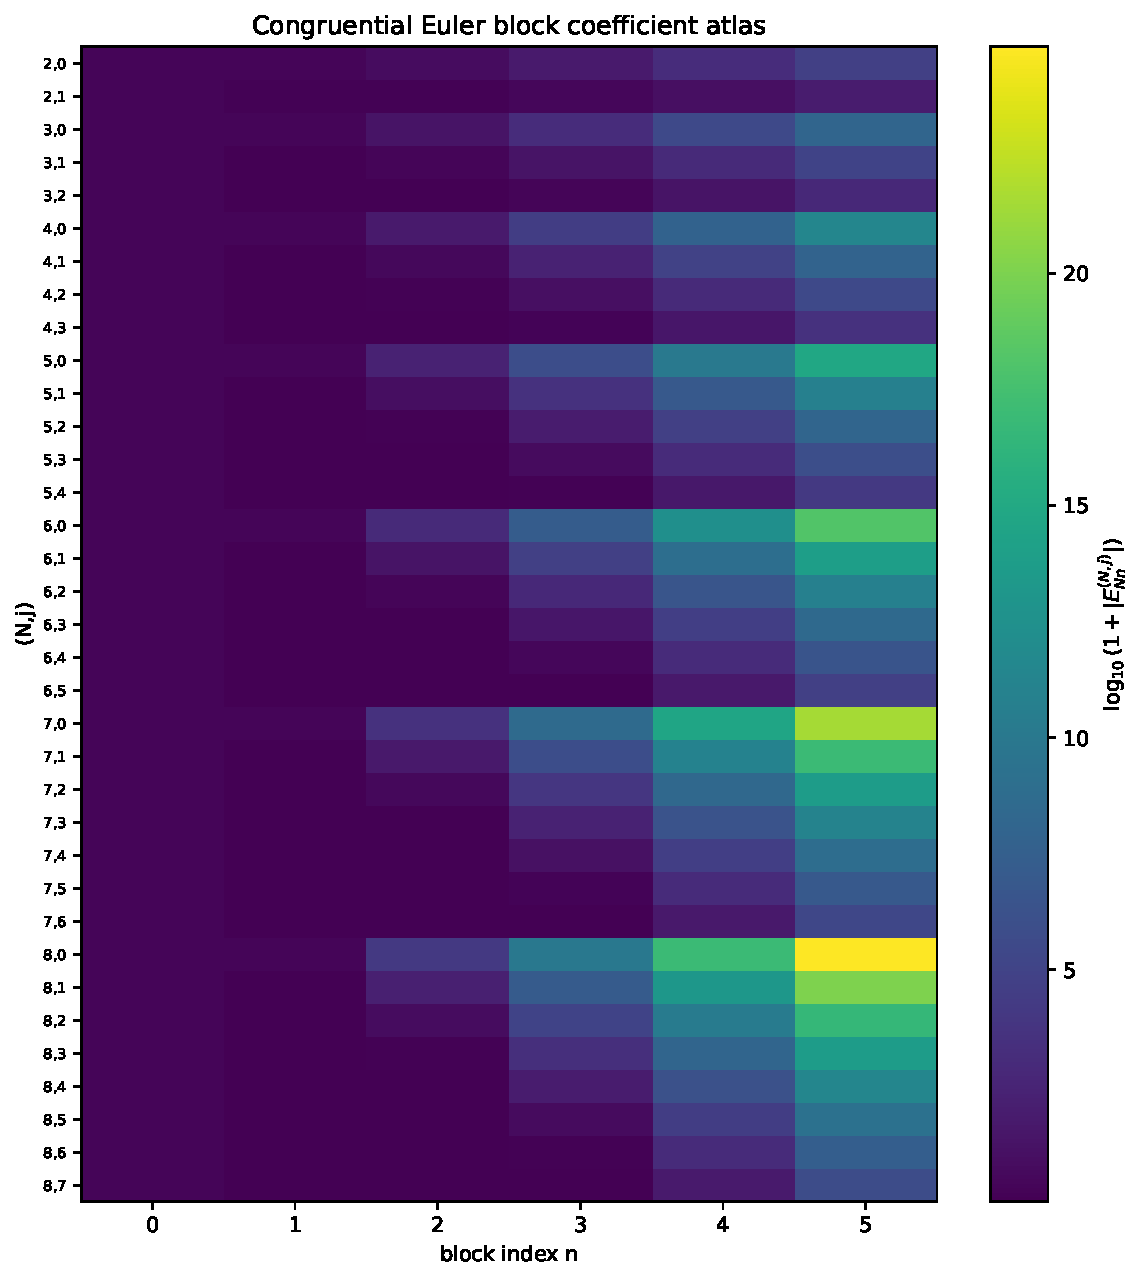
\includegraphics[width=.92\linewidth]{figures/05_congruential_euler_heatmap.pdf}
\caption{A compact coefficient atlas for many $(N,j)$ blocks.  Different residue sections generate genuinely different inverse sequences.}
\end{figure}

\paragraph{Status.}
Congruential Euler numbers now appear in recent literature, so the broad concept cannot be treated as unconditionally new.  The complete packet-calculus organization, all-class triangular system, weighted $p$-adic closure, and links to the transfer-secancy family remain substantive contributions whose exact priority must be audited carefully.

\section{Higher congruential powers and block-Appell polynomials}

\begin{definition}
For integer $r\ge0$, define
\[
\CE_{N,j}^{[r]}(z)=\CE_{N,j}(z)^r.
\]
For a complex order $\alpha$, use the germ at the origin with value $1$.
\end{definition}

The product law is immediate:
\[
\CE_{N,j}^{[r]}\CE_{N,j}^{[s]}
=\CE_{N,j}^{[r+s]}.
\]
Its coefficients therefore satisfy the same block-binomial convolution as the transfer secants.

\begin{definition}[Block-Appell polynomials]
\[
\boxed{
\CE_{N,j}(z)^r e^{xz}
=\sum_{m\ge0}E_m^{(N,j;r)}(x)\frac{z^m}{m!}.
}
\]
\end{definition}

\begin{proposition}
\[
\frac{d}{dx}E_m^{(N,j;r)}(x)
=mE_{m-1}^{(N,j;r)}(x),
\]
and
\[
E_m^{(N,j;r)}(x+y)
=\sum_{k=0}^m\binom mk
E_k^{(N,j;r)}(x)y^{m-k}.
\]
\end{proposition}

\begin{figure}[H]
\centering
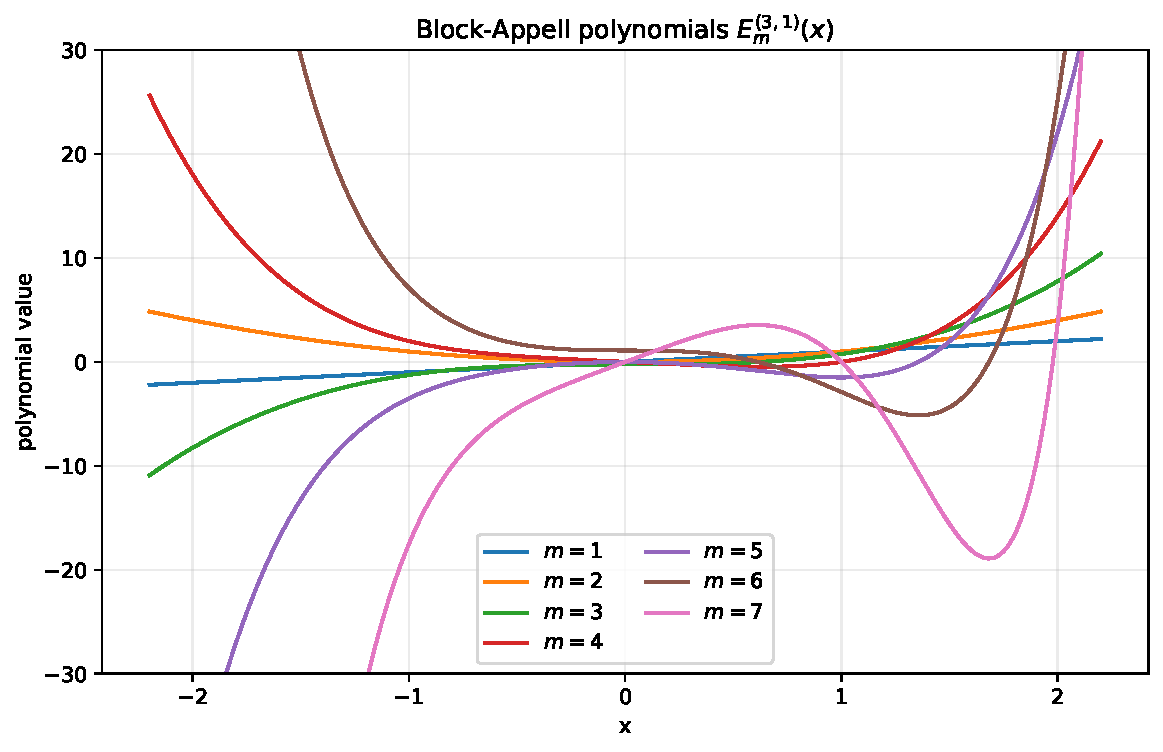
\includegraphics[width=.88\linewidth]{figures/06_block_appell_polynomials.pdf}
\caption{A low-degree slice of the $(N,j)=(3,1)$ Appell family.}
\end{figure}

\paragraph{Status.}
The Appell law is classical.  The coefficient kernel supplied by each congruential block creates a specific new or specialized Appell sequence.  The correct novelty claim concerns the parameterized family and its arithmetic structure, not Appell theory itself.

\section{Transfer-secancy parameter polynomials}

The partition formula shows that for fixed $N,n$, the coefficient of $D_N(z)^{-r}$ is a polynomial in $r$.

\begin{definition}
\[
\boxed{
P_{N,n}(r)=A_N^{[r]}(n).
}
\]
Equivalently,
\[
P_{N,n}(r)
=(Nn)!\sum_{\sum i m_i=n}
(-1)^{n+M}(r)_M
\prod_{i\ge1}\frac1{m_i!((Ni)!)^{m_i}}.
\]
\end{definition}

These polynomials are of binomial type under the block convolution:
\[
P_{N,n}(r+s)
=\sum_{q=0}^n\binom{Nn}{Nq}
P_{N,q}(r)P_{N,n-q}(s).
\]
They interpolate all integer reciprocal powers at once.

\begin{figure}[H]
\centering
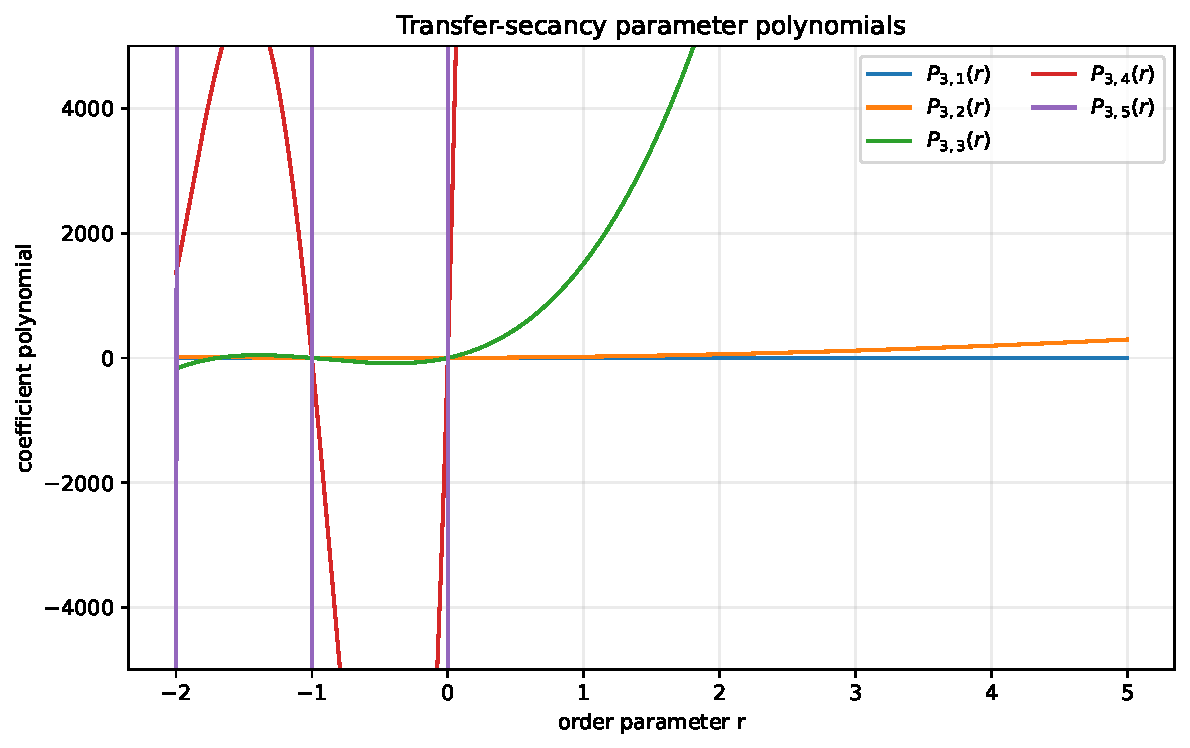
\includegraphics[width=.88\linewidth]{figures/07_secancy_parameter_polynomials.pdf}
\caption{The first parameter polynomials for $N=3$.  Integer values of $r$ recover the reciprocal-power coefficient rows.}
\end{figure}

\paragraph{Status.}
This is an explicit polynomial family generated by the calculus.  It belongs near Bell, potential, and binomial-type polynomial theory, but the $N$-block normalization and reciprocal interpretation are specific.

\section{Euler-transfer theta polynomials}

The higher-order Euler branch produces another polynomial family.

\begin{definition}
\[
\boxed{
\sech(xz)\sech^x z
=\sum_{m\ge0}\Theta_{2m}(x)\frac{z^{2m}}{(2m)!}.
}
\]
\end{definition}

The first terms are
\[
\Theta_0(x)=1,
\qquad
\Theta_2(x)=-x(x+1),
\]
\[
\Theta_4(x)=x(x+1)(5x^2+x+2),
\]
\[
\Theta_6(x)
=-x(x+1)(61x^4+14x^3+31x^2+14x+16).
\]
For higher-order Euler numbers
\[
\sech^\nu t
=\sum_{n\ge0}E_n^{\langle\nu\rangle}\frac{t^n}{n!},
\]
these polynomials are the inverse-kernel coefficients in the exact higher-order transfer.

\begin{figure}[H]
\centering
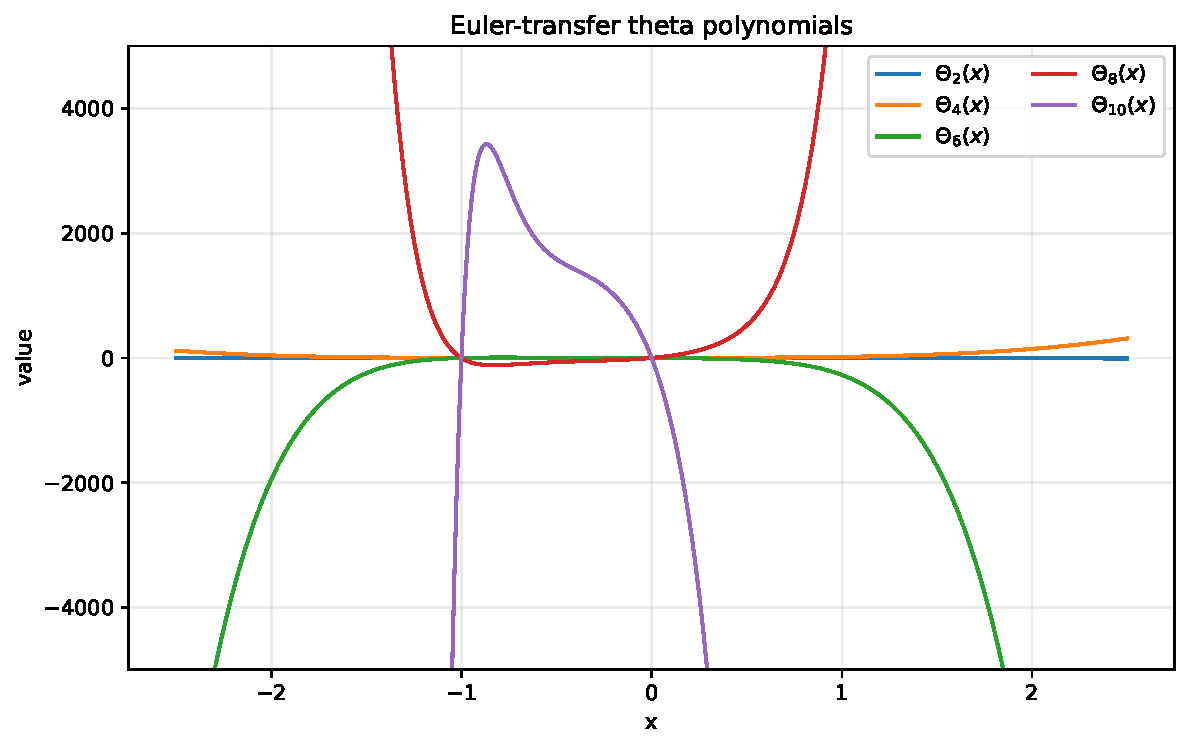
\includegraphics[width=.88\linewidth]{figures/08_theta_polynomials.pdf}
\caption{Several Euler-transfer theta polynomials.}
\end{figure}

\paragraph{Status.}
The generating function is explicit and the polynomials have integer coefficients.  A literature audit should compare them with established higher-order Euler, derivative, and potential polynomial families before a new name is fixed.

\section{Spectral block zeta functions}

Let
\[
Z_N=\{\rho\in\C:D_N(\rho)=0\},
\]
with zeros counted by multiplicity.

\begin{definition}[Formal zero zeta]
\[
\boxed{
\Zb_N(s)=\sum_{\rho\in Z_N}\rho^{-s}.
}
\]
A residue-weighted version is
\[
\boxed{
\Zb_N^{[r]}(s)
=\sum_{\rho\in Z_N}
\frac1{D_N'(\rho)^r\rho^s},
}
\]
when the zeros are simple.
\end{definition}

Several analytic choices must be fixed before these become global functions: an ordering of zeros, a branch of $\rho^{-s}$, symmetric summation, and regularization outside the initial half-plane of convergence.  These are part of the definition, not technical decorations.

For simple dominant zeros $\rho\in\mathcal P_1$, residue calculus gives
\[
A_N(n)
\sim -(Nn)!\sum_{\rho\in\mathcal P_1}
\frac1{D_N'(\rho)\rho^{Nn+1}}.
\]
For a pole of order $r$,
\[
A_N^{[r]}(n)
\sim (Nn)!\sum_{\rho\in\mathcal P_1}
\frac{(-1)^r}{D_N'(\rho)^r}
\binom{Nn+r-1}{r-1}\rho^{-Nn-r}.
\]

\begin{example}[$N=2$]
The positive zeros of $D_2(z)=\cos z$ are
\[
\rho_k=(k+\tfrac12)\pi,
\qquad k\ge0.
\]
Hence
\[
\sum_{k\ge0}\rho_k^{-s}
=\pi^{-s}\zeta(s,\tfrac12)
=\pi^{-s}(2^s-1)\zeta(s).
\]
The proposed block zeta therefore contains an ordinary Hurwitz-zeta boundary exactly.
\end{example}

\begin{example}[$N=4$]
\[
D_4(z)=\cos(z/\sqrt2)\cosh(z/\sqrt2),
\]
so its zero packets lie on the real and imaginary axes and reduce to rotated half-integer lattices.
\end{example}

\begin{figure}[H]
\centering
\begin{subfigure}{.48\linewidth}
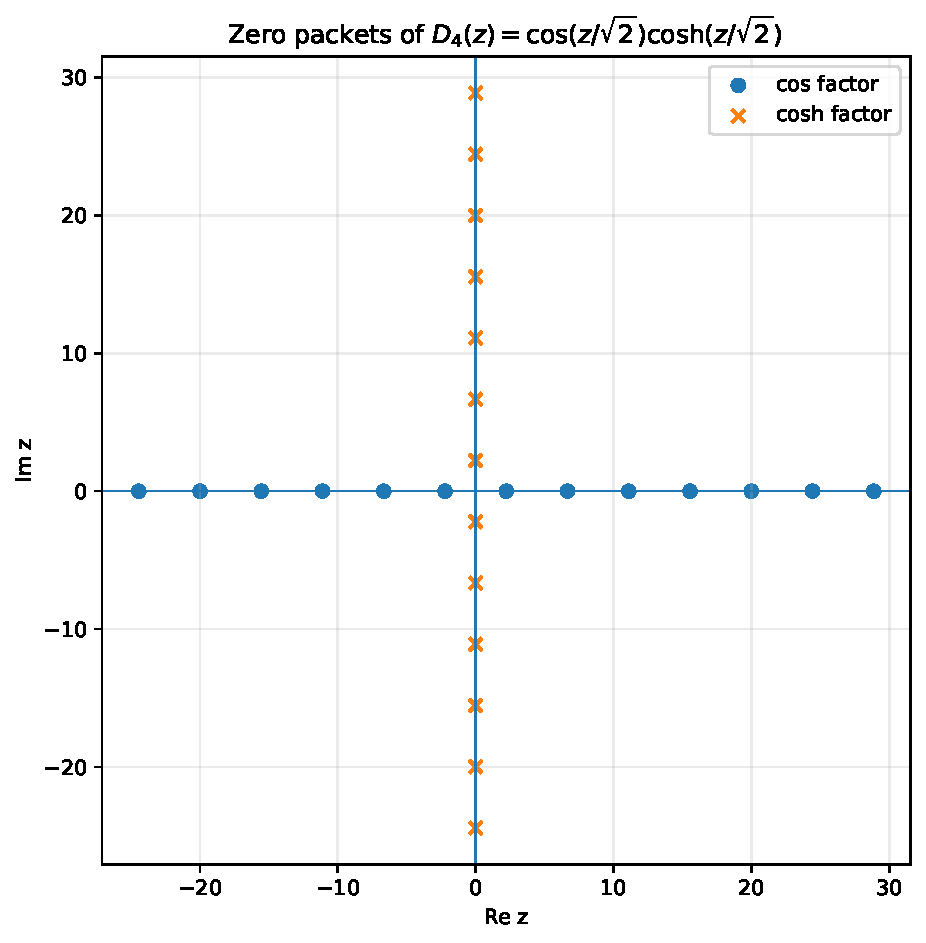
\includegraphics[width=\linewidth]{figures/09_D4_zero_packets.pdf}
\caption{The $D_4$ zero packets.}
\end{subfigure}\hfill
\begin{subfigure}{.48\linewidth}
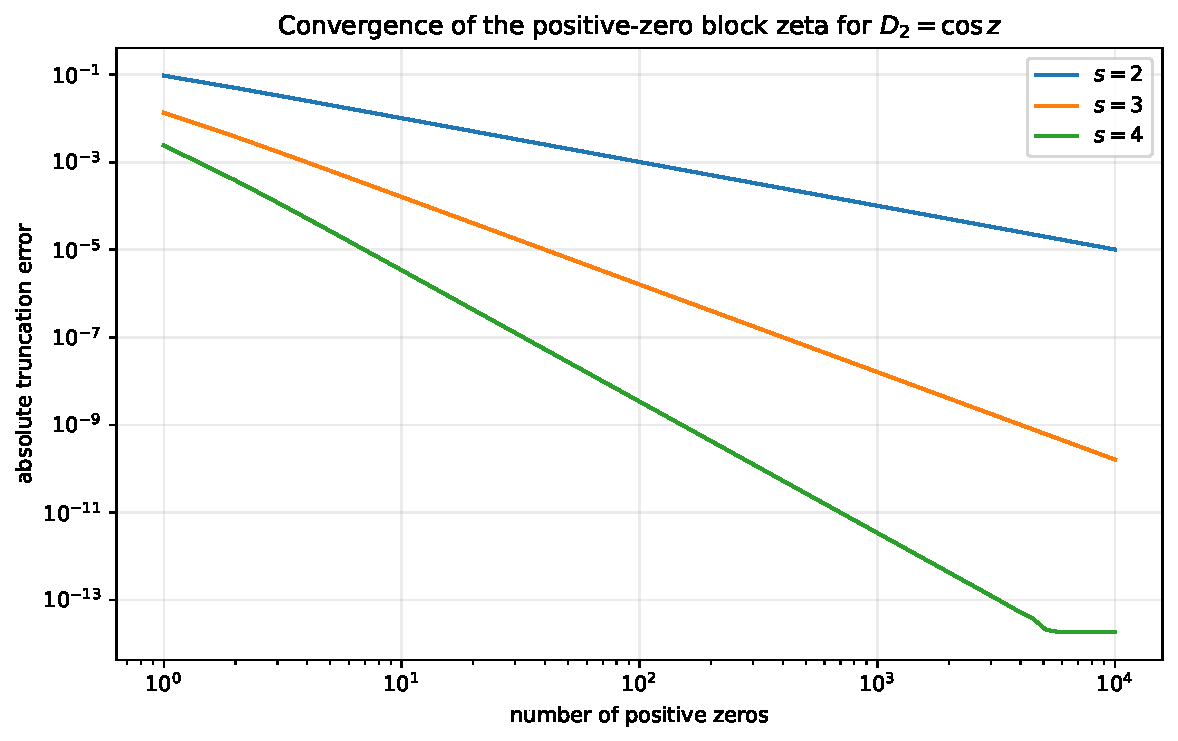
\includegraphics[width=\linewidth]{figures/10_spectral_zeta_convergence.pdf}
\caption{A convergent $D_2$ zero-zeta check.}
\end{subfigure}
\caption{The zeta family connects pole geometry to coefficient growth.}
\end{figure}

\paragraph{Status.}
This is the strongest candidate for a genuinely new analytic family, but it is also the least complete.  The registry should not promote it beyond ``zeta-type invariant'' until convergence, symmetric regularization, continuation, functional identities, and multiplicity conventions are proved.

\section{\texorpdfstring{$p$-adic transfer avatars}{p-adic transfer avatars}}

For an EGF
\[
F(t)=\sum_{n\ge0}f_n\frac{t^n}{n!},
\]
define its Amice--Mahler transform
\[
\boxed{
\widehat F(T)=F(\log(1+T)).
}
\]
The coefficients of $\widehat F$ are the Mahler-basis moments of the functional whose ordinary moments are $f_n$.

Every complex or formal family in the registry therefore has a $p$-adic avatar, for example
\[
\widehat{\Sec}_{N}^{[r]}(T)
=\Sec_N^{[r]}(\log(1+T)),
\]
\[
\widehat{\CE}_{N,j}(T)
=\CE_{N,j}(\log(1+T)).
\]
These formulas alone do not guarantee a bounded $p$-adic analytic function.  The source calculus uses either
\[
\widehat F(T)\in\Z_p[[T]]
\]
or a weighted estimate such as
\[
v_p([T^m]\widehat F)\ge-\left\lfloor\frac mp\right\rfloor.
\]
The admissible class is stable under sums, products, Euler differentiation, unit inversion, and logarithmic differentiation.  This is why the reciprocal and logarithmic-derivative functions above inherit mixed Kummer and block finite-difference statements once their transform bounds are verified.

\paragraph{Status.}
These are $p$-adic analytic or formal avatars, not automatically new special functions.  Their value lies in giving the complex families a second arithmetic realization with uniform congruence laws.

\section{Operator-valued packet functions}

The projector calculus also generates operator-valued analogues of special functions.  If $T$ is an operator and $P_i$ are packets, define
\[
f(T)_{ij}=P_i f(T)P_j.
\]
The most important example for an unbounded generator is the resolvent packet
\[
\boxed{
R_{ij}(z)=P_i(T-zI)^{-1}P_j.
}
\]
It obeys the mixed packet resolvent identity
\[
R_{ik}(z)-R_{ik}(w)
=(z-w)\sum_jR_{ij}(z)R_{jk}(w).
\]
For separated spectral clusters, contour integration produces Riesz packet functions
\[
P_r=\frac1{2\pi i}\oint_{\Gamma_r}(zI-T)^{-1}\,dz.
\]

These objects are useful and exact, but they should be called operator-valued packet functions rather than new scalar special functions.  The same distinction applies to character-projected exponentials, heat kernels, wave propagators, fractional powers, and spectral determinants.

\section{Nonlinear packet-tree functions}

For an analytic nonlinear map $F$, the $m$th derivative resolves as
\[
\mathcal J^{(m)}_{i;j_1,\ldots,j_m}
=P_iD^mF(0)[P_{j_1}\cdot,\ldots,P_{j_m}\cdot].
\]
Composition glues these tensors along rooted trees through the packet-resolved Faà di Bruno law.  Weighted analytic norms give closure under composition and local inversion.

This is a complete nonlinear function calculus, but it does not yet single out one canonical scalar special function.  Specific nonlinear equations may do so.  Examples include packet-resolved implicit functions, Volterra response functions, normal-form functions, and inverse-jet coefficients.  They belong in a future registry only after a canonical equation and normalization are fixed.

\section{Classical embeddings generated automatically}

The block operator may be applied to any analytic seed.  This automatically produces residue sections of Bessel, Airy, Mittag--Leffler, hypergeometric, polylogarithmic, theta, and orthogonal-polynomial generating functions.  These outputs can be useful, but their mere existence does not establish novelty.

For example, an ordinary power-series block of the polylogarithm is
\[
\mathcal L_{s;N,j}(z)
=\sum_{n\equiv j\, (N)}\frac{z^n}{n^s}
=\frac1N\sum_{\ell=0}^{N-1}\omega^{-j\ell}\Li_s(\omega^\ell z),
\]
which is expressible through classical polylogarithmic and Lerch functions.  The same lesson applies generally: projection may create a new coordinate representation without creating a new special function.

\section{Complete current registry}

\begingroup
\scriptsize
\setlength{\tabcolsep}{3pt}
\begin{longtable}{@{}p{.16\linewidth}p{.17\linewidth}p{.19\linewidth}p{.16\linewidth}p{.14\linewidth}@{}}
\toprule
Family & Definition & Core law & Status & Boundary\\
\midrule
\endhead
Transfer-block sections & $\mathcal B_{N,j}F$ & idempotence, reconstruction, graded product & construction schema & root-of-unity multisection\\
Transfer exponentials & $\EE_{N,j}$ & $D^Nf=\lambda^Nf$ & classical boundary & ${}_0F_{N-1}$\\
Transfer denominator & $D_N$ & $D_N^{(N)}=-D_N$ & classical boundary & generalized cosine/exponential polynomial\\
Transfer secants & $D_N^{-r}$ & power semigroup, triangular recurrence & candidate-new family & $\sec z$\\
Transfer tangents & $-D_N'/D_N$ & logarithmic derivative & explicit derived family & $\tan z$\\
Congruential Euler blocks & $(z^j/j!)/S_{N,j}$ & triangular inverse, $p$-adic laws & literature overlap; distinct packet package & Euler-family boundary\\
Higher CE powers & $\CE_{N,j}^r$ & block convolution & natural extension & higher-order Euler\\
Block-Appell polynomials & $\CE_{N,j}^re^{xz}$ & Appell derivative law & explicit derived family & Appell/Sheffer\\
Secancy polynomials & $P_{N,n}(r)$ & binomial-type parameter addition & explicit derived family & Bell/potential polynomials\\
Theta polynomials & $\sech(xz)\sech^xz$ & higher-order inverse kernel & explicit Euler-transfer family & higher-order Euler\\
Spectral block zeta & $\sum_{\rho\in Z_N}\rho^{-s}$ & zero spectrum and asymptotics & candidate-new; incomplete analysis & spectral/Hurwitz zeta\\
Residue-weighted zeta & $\sum_{\rho\in Z_N}D_N'(\rho)^{-r}\rho^{-s}$ & residue-weighted pole data & candidate-new; regularization needed & Mittag--Leffler theory\\
$p$-adic avatars & $F(\log(1+T))$ & Kummer and finite differences & conditional analytic family & Amice--Mahler\\
Packet resolvents & $P_i(T-zI)^{-1}P_j$ & mixed resolvent identity & operator-valued & resolvent/Riesz calculus\\
Nonlinear packet trees & projected jets & Faà di Bruno/operad composition & nonlinear schema & classical jet theory\\
\bottomrule
\end{longtable}
\endgroup

\begin{figure}[H]
\centering
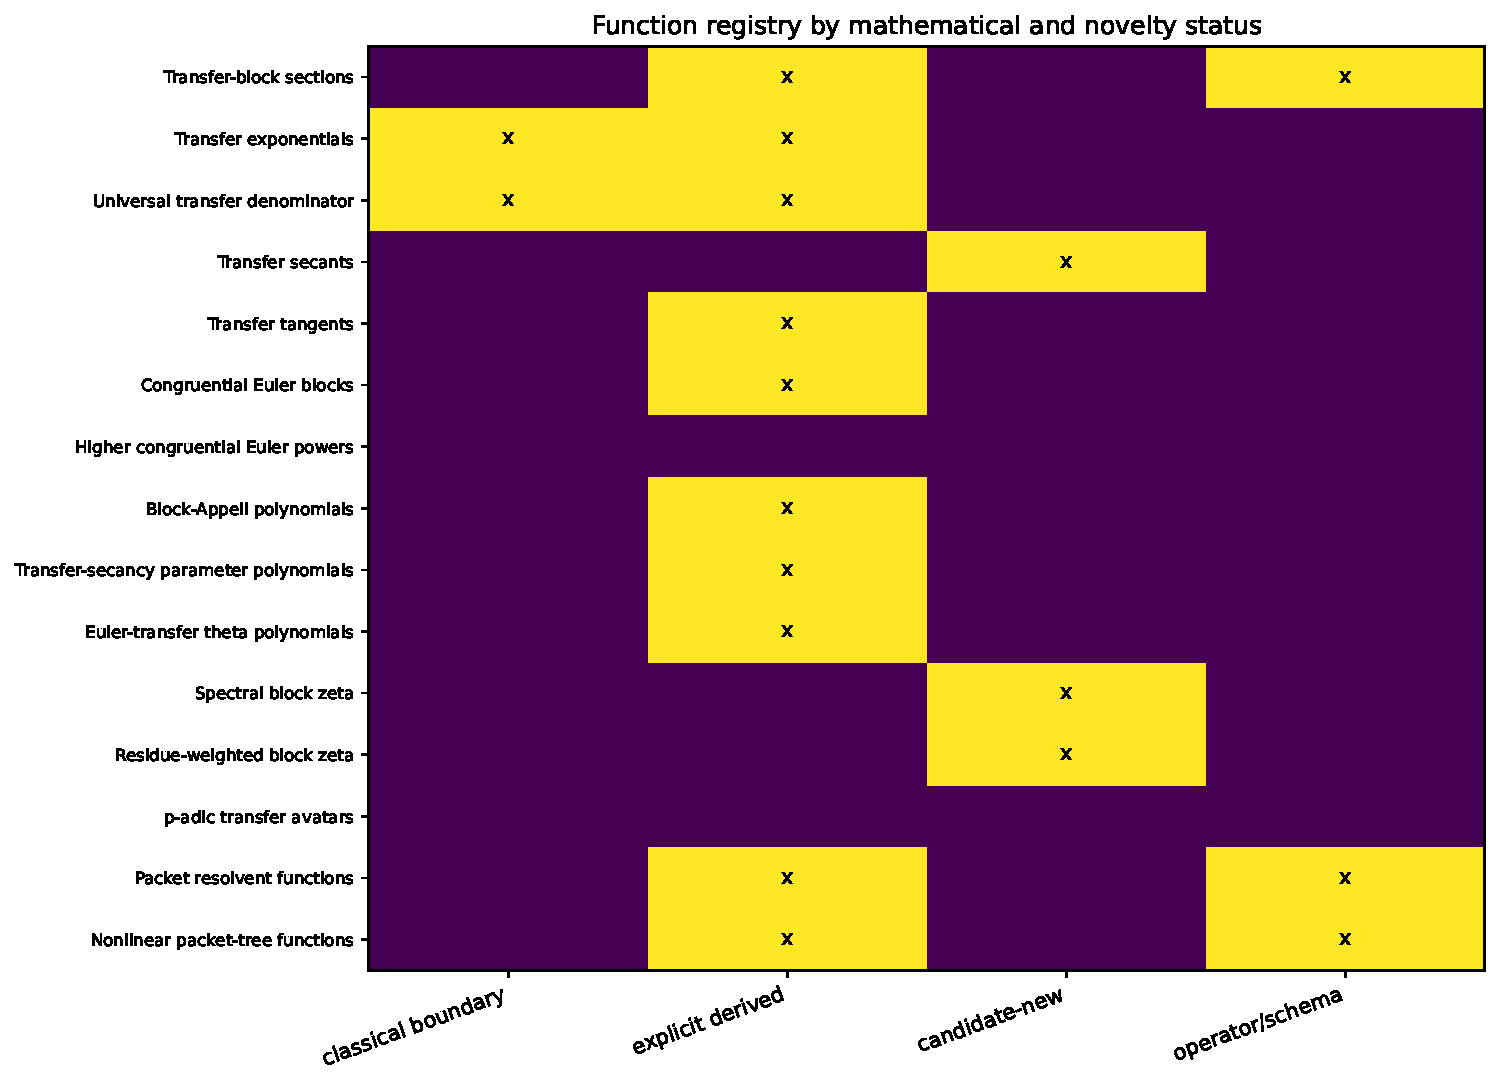
\includegraphics[width=.94\linewidth]{figures/11_registry_status_matrix.pdf}
\caption{The registry deliberately separates mathematical generation from claims of historical novelty.}
\end{figure}

\section{Novelty audit and naming policy}

A responsible naming policy should follow five rules.
\begin{enumerate}
\item Do not rename a classical multisection merely because it appears naturally in the calculus.
\item Treat a reciprocal or logarithmic derivative as a new named family only when the parameterization, coefficient law, analytic structure, and arithmetic interpretation are developed together.
\item Separate a new family from a new theorem about an existing family.
\item Mark all priority claims as provisional until databases, monographs, and historical papers have been searched by formula rather than name alone.
\item Preserve the strongest genuinely distinctive objects: the full transfer-secancy tower, congruential inverse packet family, block-Appell extension, coefficient parameter polynomials, and block zeta functions.
\end{enumerate}

The preliminary audit supports the following language.

\begin{quote}
The projector calculus generates a finite set of canonical named families and an infinite closure class.  Several seed sections are classical hypergeometric multisections.  The reciprocal-power, logarithmic-derivative, congruential inverse, packet-Appell, and zero-zeta constructions form a coherent special-function theory; some members appear new as organized families, but priority remains subject to a dedicated literature audit.
\end{quote}

\section{Computational verification}

The accompanying Python module implements exact rational recurrences for the transfer secants, transfer tangents, congruential Euler blocks, reciprocal powers, Appell polynomials, secancy parameter polynomials, and theta polynomials.  It also checks root-filter formulas, hypergeometric representations, denominator ODEs, the $D_4$ factorization, the $N=2$ block-zeta identity, and elementary Amice transforms.

The tests are designed to distinguish three levels:
\begin{enumerate}
\item exact symbolic identities;
\item high-precision analytic checks;
\item visual diagnostics that are not proofs.
\end{enumerate}

A representative code interface is:
\begin{lstlisting}[language=Python]
from special_functions import (
    secant_coefficients,
    transfer_tangent_coefficients,
    congruential_euler_coefficients,
    block_appell_polynomials,
    theta_polynomials,
)

A = secant_coefficients(N=4, order=1, nmax=10)
T = transfer_tangent_coefficients(N=4, nmax=10)
E = congruential_euler_coefficients(N=5, j=2, nmax=8)
P = block_appell_polynomials(N=5, j=2, order=1, max_degree=12)
Theta = theta_polynomials(max_m=6)
\end{lstlisting}

\section{Next mathematical priorities}

The registry is complete enough to support a focused research program.

\paragraph{First priority: analytic completion of the zeta family.}
Prove zero counting for $D_N$, choose a canonical symmetric ordering, establish the initial convergence half-plane, construct meromorphic continuation where possible, and connect regularized values to the reciprocal coefficients.

\paragraph{Second priority: differential algebra of transfer secants.}
For $N=2$, $\tan$ and $\sec$ satisfy a closed polynomial differential system.  Determine the minimal closed differential system for
\[
D_N,D_N',\ldots,D_N^{(N-1)},\Sec_N,\Tan_N.
\]
This is likely to produce higher-dimensional analogues of tangent and secant derivative polynomials.

\paragraph{Third priority: orthogonality and moment theory.}
Determine whether the block-Appell and theta polynomial families admit natural moment functionals, lowering and raising operators, Rodrigues-type formulas, or biorthogonality.

\paragraph{Fourth priority: $p$-adic interpolation.}
For each core family, determine exactly when the Amice transform is bounded, weighted, or overconvergent, and identify the associated $p$-adic measures or distributions.

\paragraph{Fifth priority: group and nonlinear extensions.}
Only promote character-filtered or nonlinear packet outputs to named special functions after a canonical scalar invariant or defining equation has been identified.

\section*{Conclusion}

The new calculus does produce special functions.  The strongest present claim is not that every displayed formula is historically new, but that the calculus supplies a coherent generator, closure algebra, coefficient theory, spectral theory, and arithmetic theory for them.  The transfer secants, transfer tangents, congruential Euler block functions, packet-Appell polynomials, parameter polynomials, theta polynomials, and spectral block zeta functions should now be treated as one documented family rather than scattered consequences.

\begin{thebibliography}{9}
\bibitem{DLMF}
NIST Digital Library of Mathematical Functions, Chapters 4 and 16, generalized hypergeometric and elementary function references.

\bibitem{Nishibuchi}
Y. Nishibuchi, preprint on $p$-adic congruences of generalized and congruential Euler numbers, arXiv:2605.10677, 2026.

\bibitem{Appell}
P. Appell, classical work on polynomial sequences defined by exponential generating functions.

\bibitem{Internal}
Komorebi P., \emph{Weighted Block-Transfer Calculus}, consolidated manuscript and formula registry.
\end{thebibliography}

\end{document}
